\documentclass[a4paper,12pt]{article}

%%% Работа с русским языком
\usepackage{cmap}					% поиск в PDF
\usepackage{mathtext} 				% русские буквы в формулах
\usepackage[T2A]{fontenc}			% кодировка
\usepackage[utf8]{inputenc}			% кодировка исходного текста
\usepackage[english,russian]{babel}	% локализация и переносы

\usepackage{amsmath,amsfonts,amssymb,amsthm,mathtools} % AMS
\usepackage{icomma} % "Умная" запятая: $0,2$ --- число, $0, 2$ --- перечисление

%%% Работа с картинками
\usepackage{graphicx}  % Для вставки рисунков
\usepackage{wrapfig} % Обтекание рисунков текстом

%%% Работа с таблицами
\usepackage{array,tabularx,tabulary,booktabs} % Дополнительная работа с таблицами
\usepackage{longtable}  % Длинные таблицы
\usepackage{multirow} % Слияние строк в таблице
\usepackage[overload]{empheq} % для рамки в формулах

%%% Страница
\usepackage{extsizes} % Возможность сделать 14-й шрифт
\usepackage{geometry} % Простой способ задавать поля
	\geometry{top=25mm}
	\geometry{bottom=35mm}
	\geometry{left=35mm}
	\geometry{right=20mm}


\begin{document}

\section{The Mean Value Theorem}

The mean value theorem is a little theoretical, and will allow us to introduce the idea of integration in a few lectures. Integration is the subject of the second half of this course. We'll use the abbreviation "MVT" when discussing it. 

Colloquially, the MVT theorem tells you that if you fly 3,000 kilometers in
6 hours, at some time during the flight you will be traveling at a speed of 500 kilometers per hour. (Because your average speed is 500 km/hr.)

The reason it's called the "mean value theorem" is because the word "mean"
is the same as the word "average".

In math symbols, it says:

\begin{empheq}[box=\fbox]{align*}
  \frac{f(b)-f(a)}{b-a}=f'(c) \text{ for some $c$, $a<c<b$} \\
  \text{Provided that $f$ is differentiable on $a<x<b$, and continuous on $a \leqslant x \leqslant b$}
\end{empheq}

\textbf{Geometric Proof of MVT}: Consider the graph of $f(x)$. Here,
$\frac{f(b)-f(a)}{b-a}$ is the slope of a secant line joining the points $(a, f (a))$ and $(b, f (b))$, and $f'(c)$ is the slope of a tangent line. We need to show that somewhere between $a$ and $b$ there's a point on the graph $(c, f (c))$ whose tangent line has the same slope
as that secant line.

\begin{figure}[ht]
\centering
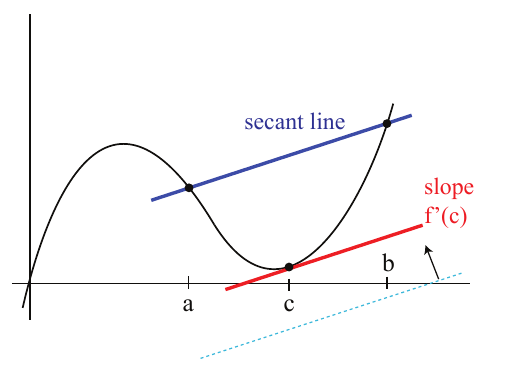
\includegraphics{fig1.png}
\caption{Illustration of the Mean Value Theorem}
\label{mvt}
\end{figure}

Take (dotted) lines parallel to the secant line, as in figure \ref{mvt} and shift them up from below the graph until one of them first touches the portion of the graph that lies between $a$ and $b$. If it does not touch, start with a dotted line above the graph and move it down until it touches.

When reading a proof, you should always be thinking about why the hypotheses are necessary. Would the proof still work if the function were discontinuous or if it were not differentiable?

We need the hypotheses that $f$ is continuous, because if you could sit still for six hours and then instantly teleport 3,000 km there would never be a time at which you were traveling 500 km/hour. The mean value theorem can't make any guarantees about discontinuous functions.

What if the function isn't differentiable? Suppose $f(x)=|x|$. Then the
dotted line always touches the graph first at $x=0$, no matter what its slope is (see figure \ref{ruinmvt}). Even though f is differentiable everywhere except $x=0$, the mean value theorem still doesn't work here; we need $f'(x)$ to exist at $all x$ between $a$ and $b$.


\begin{figure}[ht]
\centering
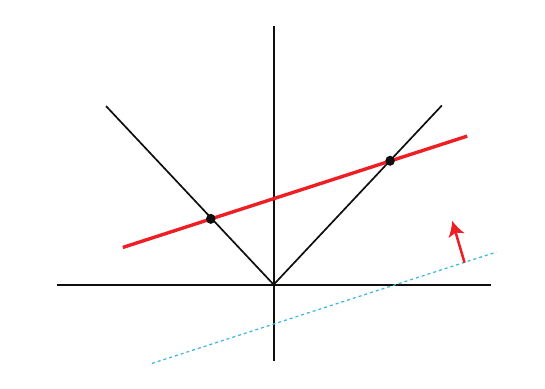
\includegraphics{fig2.png}
\caption{Graph of $y=|x|$ with secant line.(One bad point ruins the proof.)}
\label{ruinmvt}
\end{figure}

\textbf{Question}: What if the line parallel to the secant line touches the graph in more than one point?

\textbf{Answer}: The more the merrier! The graph could wiggle a lot of times and the line could touch in ten places, or f could be constant and the line could touch every point on the graph at once. In mathematics, when we claim something is true for one point we don't necessarily mean that it isn't true for others.

The fact that this point exists is a touchy point; we can see why it ought to exist but we didn't really prove that it does. The formal proof has to do with the existence of tangent lines and uses more analysis then we can do in this class.


\end{document}	